\documentclass{standalone}
\usepackage{tikz}
\usepackage{ctex,siunitx}
\setCJKmainfont{Noto Serif CJK SC}
\usepackage{tkz-euclide}
\usepackage{amsmath}
\usetikzlibrary{patterns, calc,3d}
\usetikzlibrary {decorations.pathmorphing,decorations.pathreplacing,decorations.shapes}
\tikzset{label style/.append style={font=\small}}
\begin{document}
\small
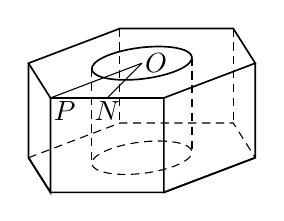
\begin{tikzpicture}[>=latex,scale=1.2,inner sep=1pt]
  \begin{scope}[z={(45:5mm)},canvas is zx plane at y=0.5]
    \draw[semithick]
      ( 30:1.2)coordinate(F)--( 90:1.2)coordinate(A)--(150:1.2)coordinate(B)--(210:1.2)coordinate(C)--(270:1.2)coordinate(D)--(330:1.2)coordinate(E)--cycle
      (0,0)circle(0.5);
    \draw(0,0)node[right]{$O$}--(210:1.2)node[below right]{$P$};
    \draw(150:1.2)--++(-90:0.6)node[below]{$N$}--(0,0);
    \coordinate (P) at ({0.5*cos(250)},{0.5*sin(250)});
    \coordinate (Q) at ({0.5*cos(70)},{0.5*sin(70)});
  \end{scope}
  \begin{scope}[z={(45:5mm)},canvas is zx plane at y=-0.5]
    \draw[semithick]
      ( 90:1.2)coordinate(A')--(150:1.2)coordinate(B')--(210:1.2)coordinate(C')--(270:1.2)coordinate(D');
    \draw[densely dashed](D')--(330:1.2)coordinate(E')--(30:1.2)coordinate(F')--(90:1.2);
    \draw[densely dashed](0,0)circle(0.5);
    \coordinate (P') at ({0.5*cos(250)},{0.5*sin(250)});
    \coordinate (Q') at ({0.5*cos(70)},{0.5*sin(70)});
  \end{scope}
  \draw[semithick](A)--(A')--(B')--(B);
  \draw[densely dashed](E)--(E')(F)--(F')(P)--(P')(Q)--(Q');
  \draw[semithick](C)--(C')--(D')--(D);
\end{tikzpicture}
\end{document}